\documentclass[notes,11pt, aspectratio=169, xcolor=table]{beamer}

\usepackage{pgfpages}
% These slides also contain speaker notes. You can print just the slides,
% just the notes, or both, depending on the setting below. Comment out the want
% you want.
\setbeameroption{hide notes} % Only slide
%\setbeameroption{show only notes} % Only notes
%\setbeameroption{show notes on second screen=right} % Both


\newtheorem{proposition}{Proposition}
\newcommand{\blue}[1]{\textcolor{blue}{#1}}
\newcommand{\white}[1]{\textcolor{white}{#1}}

\usepackage{helvet}
\usepackage[default]{lato}
\usepackage{array}
\usepackage{tikz}
\usetikzlibrary{shapes.geometric}
\usepackage{pgfplots}
\usetikzlibrary{patterns, pgfplots.fillbetween}
\usepackage{graphicx}
\usepackage{verbatim}
\setbeamertemplate{note page}{\pagecolor{yellow!5}\insertnote}
\usetikzlibrary{positioning}
\usetikzlibrary{snakes}
\usetikzlibrary{calc}
\usetikzlibrary{arrows}
\usetikzlibrary{decorations.markings}
\usetikzlibrary{shapes.misc}
\usetikzlibrary{matrix,shapes,arrows,fit,tikzmark}
\usepackage{amsmath}
\usepackage{mathpazo}
\usepackage{hyperref}
\usepackage{lipsum}
\usepackage{multimedia}
\usepackage{graphicx}
\usepackage{multirow}
\usepackage{graphicx}
\usepackage{dcolumn}
\usepackage{bbm}
\usepackage{emoji}
\usepackage[style=authoryear,sorting=nyt,uniquename=false]{biblatex}

\addbibresource{references.bib} 

\newcolumntype{d}[0]{D{.}{.}{5}}

\def\@@mybluebox[#1][#2]#3{
    \sbox\mytempbox{#3}%
    \mytemplen\ht\mytempbox
    \advance\mytemplen #1\relax
    \ht\mytempbox\mytemplen
    \mytemplen\dp\mytempbox
    \advance\mytemplen #2\relax
    \dp\mytempbox\mytemplen
    \colorbox{myblue}{\hspace{1em}\usebox{\mytempbox}\hspace{1em}}}


\usepackage{changepage}
\usepackage{appendixnumberbeamer}
\newcommand{\beginbackup}{
   \newcounter{framenumbervorappendix}
   \setcounter{framenumbervorappendix}{\value{framenumber}}
   \setbeamertemplate{footline}
   {
     \leavevmode%
     \hline
     box{%
       \begin{beamercolorbox}[wd=\paperwidth,ht=2.25ex,dp=1ex,right]{footlinecolor}%
%         \insertframenumber  \hspace*{2ex} 
       \end{beamercolorbox}}%
     \vskip0pt%
   }
 }
\newcommand{\backupend}{
   \addtocounter{framenumbervorappendix}{-\value{framenumber}}
   \addtocounter{framenumber}{\value{framenumbervorappendix}} 
}


\usepackage{graphicx}
\usepackage[space]{grffile}
\usepackage{booktabs}

% These are my colors -- there are many like them, but these ones are mine.
\definecolor{blue}{RGB}{0,114,178}
\definecolor{red}{RGB}{213,94,0}
\definecolor{yellow}{RGB}{240,228,66}
\definecolor{green}{RGB}{0,158,115}

\hypersetup{
  colorlinks=false,
  linkbordercolor = {white},
  linkcolor = {blue}
}


%% I use a beige off white for my background
\definecolor{MyBackground}{RGB}{255,253,218}

%% Uncomment this if you want to change the background color to something else
%\setbeamercolor{background canvas}{bg=MyBackground}

%% Change the bg color to adjust your transition slide background color!
\newenvironment{transitionframe}{
  \setbeamercolor{background canvas}{bg=yellow}
  \begin{frame}}{
    \end{frame}
}

\setbeamercolor{frametitle}{fg=blue}
\setbeamercolor{title}{fg=blue}
\setbeamertemplate{footline}[frame number]
\setbeamertemplate{navigation symbols}{} 
\setbeamertemplate{itemize items}{-}
\setbeamercolor{itemize item}{fg=blue}
\setbeamercolor{itemize subitem}{fg=blue}
\setbeamercolor{enumerate item}{fg=blue}
\setbeamercolor{enumerate subitem}{fg=blue}
\setbeamercolor{button}{bg=MyBackground,fg=blue,}



% If you like road maps, rather than having clutter at the top, have a roadmap show up at the end of each section 
% (and after your introduction)
% Uncomment this is if you want the roadmap!
% \AtBeginSection[]
% {
%    \begin{frame}
%        \frametitle{Roadmap of Talk}
%        \tableofcontents[currentsection]
%    \end{frame}
% }
\setbeamercolor{section in toc}{fg=blue}
\setbeamercolor{subsection in toc}{fg=red}
\setbeamersize{text margin left=1em,text margin right=1em} 

\newenvironment{wideitemize}{\itemize\addtolength{\itemsep}{10pt}}{\enditemize}

\usepackage{environ}
\NewEnviron{videoframe}[1]{
  \begin{frame}
    \vspace{-8pt}
    \begin{columns}[onlytextwidth, T] % align columns
      \begin{column}{.58\textwidth}
        \begin{minipage}[t][\textheight][t]
          {\dimexpr\textwidth}
          \vspace{8pt}
          \hspace{4pt} {\Large \sc \textcolor{blue}{#1}}
          \vspace{8pt}
          
          \BODY
        \end{minipage}
      \end{column}%
      \hfill%
      \begin{column}{.42\textwidth}
        \colorbox{green!20}{\begin{minipage}[t][1.2\textheight][t]
            {\dimexpr\textwidth}
            Face goes here
          \end{minipage}}
      \end{column}%
    \end{columns}
  \end{frame}
}

\title[]{International Trade: Lecture 10}
\subtitle[]{Distribution of Income and the Political Economy of Trade Policy}
\author[Góes]
{Carlos Góes\inst{1}}
\date{Fall 2025}
\institute[GWU]{\inst{1} George Washington University }



\begin{document}

%%% TIKZ STUFF
\tikzset{   
        every picture/.style={remember picture,baseline},
        every node/.style={anchor=base,align=center,outer sep=1.5pt},
        every path/.style={thick},
        }
\newcommand\marktopleft[1]{%
    \tikz[overlay,remember picture] 
        \node (marker-#1-a) at (-.3em,.3em) {};%
}
\newcommand\markbottomright[2]{%
    \tikz[overlay,remember picture] 
        \node (marker-#1-b) at (0em,0em) {};%
}
\tikzstyle{every picture}+=[remember picture] 
\tikzstyle{mybox} =[draw=black, very thick, rectangle, inner sep=10pt, inner ysep=20pt]
\tikzstyle{fancytitle} =[draw=black,fill=red, text=white]
%%%% END TIKZ STUFF



%----------------------------------------------------------------------%
%-------------------       TITLE PAGE       ---------------------------%
%----------------------------------------------------------------------%





%----------------------------------------------------------------------%






%----------------------------------------------------------------------%
%----------------------------------------------------------------------%

%----------------------------------------------------------------------%
\frame{\titlepage}
\addtocounter{framenumber}{-1}
%----------------------------------------------------------------------%



%----------------------------------------------------------------------%
%----------------------------------------------------------------------%

\section{Intro and recap}

\begin{frame}{Last class}
\begin{wideitemize}
    \item Specifics Factor Model (Ricardo-Viner)
    \item Can analyze consequences of
    \begin{itemize}
        \item Productivity shocks
        \item Changes in factor endowments 
    \end{itemize}
    \item In most cases, results are intuitive:
    \begin{itemize}
        \item ``Dutch disease'' (Boom in export sectors, Bids up wages, which leads to a contraction in the other sectors)
        \item Useful political-economy applications (Grossman and Helpman 1994)
    \end{itemize}
    \item Easy to extend the analysis to more than 2 sectors:
    \begin{itemize}
        \item Plot labor demand in one sector vs. rest of the economy
        \item Convenient for empirical work (Kovak 2013) 
    \end{itemize}
    
    \item 
\end{wideitemize}
\end{frame}

\section{Distribution of income}

\begin{frame}{Distribution of income: Diagram}

\begin{figure}[htp]
    \centering
    \begin{tikzpicture}
    
    % Setup axis
    \begin{axis}[
        axis lines=middle,
        xtick=\empty,
        ytick=\empty,
        xmin=0, xmax=2.2,
        ymin=0, ymax=1.2,
        samples=300,
        axis line style={->},
        width=12cm,
        height=8cm,
        domain=0.05:1.05,
        clip=false,
    ]
    
    \pgfmathsetmacro{\Pm}{1}
    \pgfmathsetmacro{\beta}{0.5}
    \pgfmathsetmacro{\Zm}{1}
    \pgfmathsetmacro{\K}{1}
    
    \pgfmathsetmacro{\Pa}{1}
    \pgfmathsetmacro{\beta}{0.5}
    \pgfmathsetmacro{\Za}{1}
    \pgfmathsetmacro{\T}{1}
    
    \pgfmathsetmacro{\Omega}{(\Pm*\Zm / \Pa*\Za)^(1/\beta) * \K / \T}
    \pgfmathsetmacro{\L}{2.2}
    
    \pgfmathsetmacro{\Ls}{ \Omega / (1+\Omega) * \L}
    \pgfmathsetmacro{\ws}{ \Pm * \Zm * (1-\beta) * (\K / \Ls )^(\beta) }
    
    
    
    
    \addplot[->] coordinates {(2.2,0) (2.2,1.2)};
    \addplot[->] coordinates {(2.2,0) (0,0)};
    
    
    % Demand in manufacturing (left)
    \addplot[domain=0.2:2.2, thick, red] (x, {\Pm * \Zm * (1-\beta) * (\K / x)^(\beta)});
    \node[align=left, anchor=north west, red!70] at (axis cs:0.2,0.65) {\scriptsize Manufacturing \\ \scriptsize producers income };
    \node[black, P] at (axis cs:-0.25,1.15) {\scriptsize $w_i$, \textcolor{red}{$P_M \times MPL_{i,M}$}};
    \node[black] at (axis cs:0,-0.04) {\scriptsize $0~(\bar{L}_i)$};

    % Demand in food (right)
    \addplot[domain=0.2:2.2, thick, blue] (2.2-x, {(\Pm * \Zm * (1-\beta) * (\K / x)^(\beta)});
    \node[align=right, anchor=north east, blue!70] at (axis cs:2.2-0.2,0.65) {\scriptsize Agricultural \\ \scriptsize producers income };
    \node[black, P] at (axis cs:2.2+0.25,1.15) {\scriptsize $w_i$, \textcolor{blue}{$P_A \times MPL_{i,A}$}};
    \node[black] at (axis cs:2.2,-0.04) {\scriptsize $\bar{L}_i~(0)$};
    
    % Equilibrium point
    \addplot[dashed] coordinates {(0,\ws) (2.2,\ws)};
    \addplot[mark=*, black, mark size=1.5pt] coordinates {(\Ls,\ws)};
    \addplot[dashed] coordinates {(\Ls,0) (\Ls,\ws)};
    \node[below] at (axis cs:\Ls,-0.02) {\small $L_M = \bar{L} - L_F$};
    \node[black, P] at (axis cs:-0.05,\ws) {\scriptsize $w_i^*$};
    \node[black, P] at (axis cs:2.2+0.05,\ws) {\scriptsize $w_i^*$};  
    \node[align=center, anchor=north, black!70] at (axis cs:1.1,0.35) {\small Workers' \text{      } income};

    % Fillings
        % manufacturing producer
        \addplot [
        name path=A,
        domain=0.2:\Ls,
        draw=none
        ] (x, {\Pm * \Zm * (1-\beta) * (\K / x)^(\beta)});
    
        \path[name path=B] (axis cs:0.2,\ws) -- (axis cs:\Ls,\ws);
    
        \addplot [
            fill=red!20,
            draw=none
            ] fill between [of=A and B];

        % agricultural producer
        \addplot [
        name path=C,
        domain=0.2:\Ls,
        draw=none
        ] (2.2-x, {(\Pm * \Zm * (1-\beta) * (\K / x)^(\beta)});
    
        \path[name path=D] (axis cs:\Ls,\ws) -- (axis cs:2.2-0.2,\ws);
    
        \addplot [
            fill=blue!20,
            draw=none
            ] fill between [of=C and D];

        % workers
        \addplot [
        name path=E,
        domain=0.2:2,
        draw=none
        ] (x,\ws);
    
        \path[name path=F] (axis cs:0.2,0) -- (axis cs:2.2-0.2,0);
    
        \addplot [
            fill=black!20,
            draw=none
            ] fill between [of=E and F];


    \end{axis}
    \end{tikzpicture}
\end{figure}
    
\end{frame}


\begin{frame}{Trade Equilibrium: Labor Market Shifts}
    \centering
    \begin{tikzpicture}
    
    % Setup axis
    \begin{axis}[
        axis lines=middle,
        xtick=\empty,
        ytick=\empty,
        xmin=0, xmax=2.2,
        ymin=0, ymax=1.2,
        samples=300,
        axis line style={->},
        width=12cm,
        height=8cm,
        domain=0.05:1.05,
        clip=false,
    ]
    \pgfmathsetmacro{\beta}{1/3}
    \pgfmathsetmacro{\alpha}{1/2}

    \pgfmathsetmacro{\Zm}{1}
    \pgfmathsetmacro{\K}{1}
    
    \pgfmathsetmacro{\Za}{1}
    \pgfmathsetmacro{\T}{1}

    \pgfmathsetmacro{\Kf}{1}
    \pgfmathsetmacro{\Tf}{8}


    \pgfmathsetmacro{\P}{\Za/\Zm * ((1-\alpha)/\alpha * \T / \K)^(\beta)}   
    \pgfmathsetmacro{\Pw}{\Za/\Zm * ((1-\alpha)/\alpha * ( ( \T + \Tf) / (\K+\Kf ) )^(\beta)}  

    \pgfmathsetmacro{\L}{2.2}
    \pgfmathsetmacro{\Omega}{(\P *\Zm / \Za)^(1/\beta) * \K / \T}      
    \pgfmathsetmacro{\Ls}{ \Omega / (1+\Omega) * \L}    
    \pgfmathsetmacro{\ws}{ \P * \Zm * (1-\beta) * (\K / \Ls )^(\beta) }

    
    \pgfmathsetmacro{\Omegaw}{(\Pw *\Zm / \Za)^(1/\beta) * \K / \T}      
    \pgfmathsetmacro{\Lsw}{ \Omegaw / (1+\Omegaw) * \L}    
    \pgfmathsetmacro{\wsw}{ \Pw * \Zm * (1-\beta) * (\K / \Lsw )^(\beta) }   
    
    
    \addplot[->] coordinates {(2.2,0) (2.2,1.2)};
    \addplot[->] coordinates {(2.2,0) (0,0)};
    
    
    % Demand in manufacturing (left)
    \addplot[domain=0.2:2.2, thick, red] (x, {\P * \Zm * (1-\beta) * (\K / x)^(\beta)});
    %\node[align=center, anchor=north west, red!70] at (axis cs:0.2,0.65) {\small $P_M \times MPL_{i,M}$};
    \node[black, P] at (axis cs:-0.25,1.15) {\scriptsize $w_i$, \textcolor{red}{$P_M \times MPL_{i,M}$}};
    \node[black] at (axis cs:0,-0.04) {\scriptsize $0~(\bar{L}_i)$};
    
    % Demand in food (right)
    \addplot[domain=0.2:2.2, thick, blue] (2.2-x, {(\Za * (1-\beta) * (\T / x)^(\beta)});
    %\node[align=center, anchor=north east, blue!70] at (axis cs:2.2-0.2,0.65) {\small $P_A \times MPL_{i,A}$};
    \node[black, P] at (axis cs:2.2+0.25,1.15) {\scriptsize $w_i$, \textcolor{blue}{$P_A \times MPL_{i,A}$}};
    \node[black] at (axis cs:2.2,-0.04) {\scriptsize $\bar{L}_i~(0)$};
    
    % Equilibrium point
    \addplot[dashed] coordinates {(0,\ws) (2.2,\ws)};
    \addplot[dashed] coordinates {(\Ls,0) (\Ls,\ws)};
    \addplot[mark=*, mark size=1.5pt] coordinates {(\Ls,\ws)};
    \node[below] at (axis cs:\Ls,-0.02) {\small $L_M$};
    \node[black, P] at (axis cs:-0.05,\ws) {\scriptsize $w_i^*$};
    \node[black, P] at (axis cs:2.2+0.05,\ws) {\scriptsize $w_i^*$};

    % Bottom left and right axis labels
    %\node[below] at (axis cs:-0.5,-0.02) {\scriptsize $L_M$};
    %\node[below] at (axis cs:0.5,-0.02) {\scriptsize $L - L_M~(= L_F)$};
    
    \end{axis}
    
    \end{tikzpicture}
\end{frame}

\begin{frame}{Trade Equilibrium: Labor Market Shifts}
\addtocounter{framenumber}{-1}
    \centering
    \begin{tikzpicture}
    
    % Setup axis
    \begin{axis}[
        axis lines=middle,
        xtick=\empty,
        ytick=\empty,
        xmin=0, xmax=2.2,
        ymin=0, ymax=1.2,
        samples=300,
        axis line style={->},
        width=12cm,
        height=8cm,
        domain=0.05:1.05,
        clip=false,
    ]
    \pgfmathsetmacro{\beta}{1/3}
    \pgfmathsetmacro{\alpha}{1/2}

    \pgfmathsetmacro{\Zm}{1}
    \pgfmathsetmacro{\K}{1}
    
    \pgfmathsetmacro{\Za}{1}
    \pgfmathsetmacro{\T}{1}

    \pgfmathsetmacro{\Kf}{1}
    \pgfmathsetmacro{\Tf}{8}


    \pgfmathsetmacro{\P}{\Za/\Zm * ((1-\alpha)/\alpha * \T / \K)^(\beta)}   
    \pgfmathsetmacro{\Pw}{\Za/\Zm * ((1-\alpha)/\alpha * ( ( \T + \Tf) / (\K+\Kf ) )^(\beta)}  

    \pgfmathsetmacro{\L}{2.2}
    \pgfmathsetmacro{\Omega}{(\P *\Zm / \Za)^(1/\beta) * \K / \T}      
    \pgfmathsetmacro{\Ls}{ \Omega / (1+\Omega) * \L}    
    \pgfmathsetmacro{\ws}{ \P * \Zm * (1-\beta) * (\K / \Ls )^(\beta) }

    
    \pgfmathsetmacro{\Omegaw}{(\Pw *\Zm / \Za)^(1/\beta) * \K / \T}      
    \pgfmathsetmacro{\Lsw}{ \Omegaw / (1+\Omegaw) * \L}    
    \pgfmathsetmacro{\wsw}{ \Pw * \Zm * (1-\beta) * (\K / \Lsw )^(\beta) }   
    
    
    \addplot[->] coordinates {(2.2,0) (2.2,1.2)};
    \addplot[->] coordinates {(2.2,0) (0,0)};
    
    
    % Demand in manufacturing (left)
    \addplot[domain=0.2:2.2, thick, red!50] (x, {\P * \Zm * (1-\beta) * (\K / x)^(\beta)});
    % Demand in manufacturing (left)
    \addplot[domain=0.7:2.2, thick, red] (x, {\Pw * \Zm * (1-\beta) * (\K / x)^(\beta)});
    %\node[align=center, anchor=north west, red!70] at (axis cs:0.2,0.65) {\small $P_M \times MPL_{i,M}$};
    \node[black, P] at (axis cs:-0.25,1.15) {\scriptsize $w_i$, \textcolor{red}{$P_M \times MPL_{i,M}$}};
    \node[black] at (axis cs:0,-0.04) {\scriptsize $0~(\bar{L}_i)$};
    
    % Demand in food (right)
    \addplot[domain=0.2:2.2, thick, blue] (2.2-x, {(\Za * (1-\beta) * (\T / x)^(\beta)});
    %\node[align=center, anchor=north east, blue!70] at (axis cs:2.2-0.2,0.65) {\small $P_A \times MPL_{i,A}$};
    \node[black, P] at (axis cs:2.2+0.25,1.15) {\scriptsize $w_i$, \textcolor{blue}{$P_A \times MPL_{i,A}$}};
    \node[black] at (axis cs:2.2,-0.04) {\scriptsize $\bar{L}_i~(0)$};
    
    % Equilibrium point
    \addplot[dashed, gray] coordinates {(0,\ws) (2.2,\ws)};
    \addplot[mark=*, gray, mark size=1.5pt] coordinates {(\Ls,\ws)};
    \addplot[mark=*, gray, mark size=1.5pt] coordinates {(\Ls,{\Pw * \Zm * (1-\beta)*(\K/\Ls)^(\beta)})};
    \addplot[dashed, gray] coordinates {(\Ls,0) (\Ls, {\Pw * \Zm * (1-\beta)*(\K/\Ls)^(\beta)})};
    \node[below] at (axis cs:\Ls,-0.02) {\small $L_M$};
    \node[black, P] at (axis cs:-0.05,\ws) {\scriptsize $w_i^*$};
    \node[black, P] at (axis cs:2.2+0.05,\ws) {\scriptsize $w_i^*$};

        \addplot[dashed] coordinates {(0,\wsw) (2.2,\wsw)};
    \addplot[mark=*, black, mark size=1.5pt] coordinates {(\Lsw,\wsw)};
    \addplot[dashed] coordinates {(\Lsw,0) (\Lsw,\wsw)};
    \node[below] at (axis cs:\Lsw,-0.02) {\small $(L_M)^{Trade}$};
    \node[black, P] at (axis cs:-0.12,\wsw) {\scriptsize $(w_i^*)^{Trade}$};
    \node[black, P] at (axis cs:2.2+0.12,\wsw) {\scriptsize $(w_i^*)^{Trade}$};

    % Bottom left and right axis labels
    %\node[below] at (axis cs:-0.5,-0.02) {\scriptsize $L_M$};
    %\node[below] at (axis cs:0.5,-0.02) {\scriptsize $L - L_M~(= L_F)$};
    
    \end{axis}
    
    \end{tikzpicture}
\end{frame}


\begin{frame}{Trade Equilibrium: Labor Market Shifts}
\addtocounter{framenumber}{-1}
\centering
    \begin{tikzpicture}
    
    % Setup axis
    \begin{axis}[
        axis lines=middle,
        xtick=\empty,
        ytick=\empty,
        xmin=0, xmax=2.2,
        ymin=0, ymax=1.2,
        samples=300,
        axis line style={->},
        width=12cm,
        height=8cm,
        domain=0.05:1.05,
        clip=false,
    ]
    \pgfmathsetmacro{\beta}{1/3}
    \pgfmathsetmacro{\alpha}{1/2}

    \pgfmathsetmacro{\Zm}{1}
    \pgfmathsetmacro{\K}{1}
    
    \pgfmathsetmacro{\Za}{1}
    \pgfmathsetmacro{\T}{1}

    \pgfmathsetmacro{\Kf}{1}
    \pgfmathsetmacro{\Tf}{8}

    \pgfmathsetmacro{\P}{\Za/\Zm * ((1-\alpha)/\alpha * \T / \K)^(\beta)}   
    \pgfmathsetmacro{\Pw}{\Za/\Zm * ((1-\alpha)/\alpha * ( ( \T + \Tf) / (\K+\Kf ) )^(\beta)}  

    \pgfmathsetmacro{\L}{2.2}
    \pgfmathsetmacro{\Omega}{(\P *\Zm / \Za)^(1/\beta) * \K / \T}      
    \pgfmathsetmacro{\Ls}{ \Omega / (1+\Omega) * \L}    
    \pgfmathsetmacro{\ws}{ \P * \Zm * (1-\beta) * (\K / \Ls )^(\beta) }

    \pgfmathsetmacro{\Omegaw}{(\Pw *\Zm / \Za)^(1/\beta) * \K / \T}      
    \pgfmathsetmacro{\Lsw}{ \Omegaw / (1+\Omegaw) * \L}    
    \pgfmathsetmacro{\wsw}{ \Pw * \Zm * (1-\beta) * (\K / \Lsw )^(\beta) }   

    \addplot[->] coordinates {(2.2,0) (2.2,1.2)};
    \addplot[->] coordinates {(2.2,0) (0,0)};

    % Demand in manufacturing (left)
    \addplot[domain=0.2:2.2, thick, red!50] (x, {\P * \Zm * (1-\beta) * (\K / x)^(\beta)});
    \addplot[domain=0.7:2.2, thick, red] (x, {\Pw * \Zm * (1-\beta) * (\K / x)^(\beta)});
    \node[black, P] at (axis cs:-0.25,1.15) {\scriptsize $w_i$, \textcolor{red}{$P_M \times MPL_{i,M}$}};
    \node[black] at (axis cs:0,-0.04) {\scriptsize $0~(\bar{L}_i)$};

    % Demand in food (right)
    \addplot[domain=0.2:2.2, thick, blue] (2.2-x, {(\Za * (1-\beta) * (\T / x)^(\beta)});
    \node[black, P] at (axis cs:2.2+0.25,1.15) {\scriptsize $w_i$, \textcolor{blue}{$P_A \times MPL_{i,A}$}};
    \node[black] at (axis cs:2.2,-0.04) {\scriptsize $\bar{L}_i~(0)$};

    % Equilibrium point
    \addplot[dashed, gray] coordinates {(0,\ws) (2.2,\ws)};
    \addplot[mark=*, gray, mark size=1.5pt] coordinates {(\Ls,\ws)};
    \addplot[mark=*, gray, mark size=1.5pt] coordinates {(\Ls,{\Pw * \Zm * (1-\beta)*(\K/\Ls)^(\beta)})};
    \addplot[dashed, gray] coordinates {(\Ls,0) (\Ls, {\Pw * \Zm * (1-\beta)*(\K/\Ls)^(\beta)})};
    \node[below] at (axis cs:\Ls,-0.02) {\small $L_M$};
    \node[black, P] at (axis cs:-0.05,\ws) {\scriptsize $w_i^*$};
    \node[black, P] at (axis cs:2.2+0.05,\ws) {\scriptsize $w_i^*$};

    \addplot[dashed] coordinates {(0,\wsw) (2.2,\wsw)};
    \addplot[mark=*, black, mark size=1.5pt] coordinates {(\Lsw,\wsw)};
    \addplot[dashed] coordinates {(\Lsw,0) (\Lsw,\wsw)};
    \node[below] at (axis cs:\Lsw,-0.02) {\small $(L_M)^{Trade}$};
    \node[black, P] at (axis cs:-0.12,\wsw) {\scriptsize $(w_i^*)^{Trade}$};
    \node[black, P] at (axis cs:2.2+0.12,\wsw) {\scriptsize $(w_i^*)^{Trade}$};

    % Horizontal brace with label
    \draw [decorate,decoration={brace,mirror,amplitude=4pt},yshift=-20pt]
          (axis cs:\Ls,0) -- (axis cs:\Lsw,0) 
          node[midway,below,yshift=-2pt] {\scriptsize Labor moved from $A$ to $M$};

    % Vertical brace for change in PM*MPL
    \draw [decorate,decoration={brace,amplitude=4pt},xshift=-4pt]
          (axis cs:\Ls,\ws) -- (axis cs:\Ls,{\Pw * \Zm * (1-\beta)*(\K/\Ls)^(\beta)}) 
          node[midway,left=3pt] {$\substack{\text{Change in} \\ P_M \times MPL_{i,M}}$};

    % Vertical brace for change in wages
    \draw [decorate,decoration={brace, mirror,amplitude=4pt},xshift=8pt]
          (axis cs:\Ls,\ws) -- (axis cs:\Ls,\wsw) 
          node[midway,right=4pt] {$\substack{\text{Change} \\ \text{in wages}}$
          };

    \end{axis}
    \end{tikzpicture}
\end{frame}

\begin{frame}{Distributional effects of trade}
    \begin{wideitemize}
    \item Wage paid to workers increases, but less than proportionally compared to the increase in the price of manufacturing goods ($P_M$)
    \begin{itemize}
        \item Real wage in terms of manufactures, $w/P_M$, declines, while the real wage in terms of food, $w/P_A$, increases. 
        \item Net impact on workers' welfare is ambiguous -- it depends on how much they consume of each good, which in turn reflects their preferences. 
    \end{itemize}
    \item<2-> Capital owners unambiguously gain
    \begin{itemize}
        \item real wage in terms of manufacturing good has fallen, surplus accruing to capital
        \item increase in real income—both in terms of manufactured goods and foodstuff
    \end{itemize}
    \item<3-> Landowners unambiguously lose
    \begin{itemize}
        \item real wage in terms of food has risen, reducing the residual income
        \item relative price of manufacturing goods has increased, lowering purchasing power on land rents
    \end{itemize}

    \end{wideitemize}
\end{frame}


\begin{frame}{Distributional effects of trade}
    We can summarize the distributional effects of a relative price change as follows:
    \vspace{12pt}
    \begin{wideitemize}
        \item The specific factor employed in the sector with a rising relative price gains.
        \item The specific factor employed in the sector with a falling relative price loses.
        \item The mobile factor (labor) experiences an ambiguous welfare effect.
    \end{wideitemize}
\end{frame}

\begin{frame}{While there are distributional effects, there are aggregate gains}
\begin{figure}
    \centering
    \begin{tikzpicture}
    \pgfmathsetmacro{\beta}{1/3}
    \pgfmathsetmacro{\alpha}{0.5}

    \pgfmathsetmacro{\Zm}{1}
    \pgfmathsetmacro{\K}{1}
    
    \pgfmathsetmacro{\Za}{1}
    \pgfmathsetmacro{\T}{1}

    \pgfmathsetmacro{\Kf}{1}
    \pgfmathsetmacro{\Tf}{15}


    \pgfmathsetmacro{\P}{\Za/\Zm * ((1-\alpha)/\alpha * \T / \K)^(\beta)}   


    \pgfmathsetmacro{\Pw}{\Za/\Zm * ((1-\alpha)/\alpha * ( ( \T + \Tf) / (\K+\Kf ) )^(\beta)}  
    \pgfmathsetmacro{\Qw}{(1-\alpha)/\alpha / \Pw}

    \pgfmathsetmacro{\L}{1}
    \pgfmathsetmacro{\Omega}{(\P *\Zm / \Za)^(1/\beta) * \K / \T}      
    \pgfmathsetmacro{\Ls}{ \Omega / (1+\Omega) * \L}    
    \pgfmathsetmacro{\Ym}{ \Zm * \K^(\beta) * \Ls^(1-\beta) }
    \pgfmathsetmacro{\Ya}{ \Za * \T^(\beta) * (1-\Ls)^(1-\beta) }

    \pgfmathsetmacro{\Omegaw}{(\Pw *\Zm / \Za)^(1/\beta) * \K / \T}      
    \pgfmathsetmacro{\Lsw}{ \Omegaw / (1+\Omegaw) * \L}    
    \pgfmathsetmacro{\Ymw}{ \Zm * \K^(\beta) * \Lsw^(1-\beta) }
    \pgfmathsetmacro{\Yaw}{ \Za * \T^(\beta) * (1-\Lsw)^(1-\beta) }
    \pgfmathsetmacro{\Iw}{ \Pw * \Ymw + \Yaw }
    \pgfmathsetmacro{\Qaw}{(1-\alpha) * \Iw}
    \pgfmathsetmacro{\Qmw}{(\alpha)/\Pw * \Iw}

%    \pgfmathsetmacro{\ws}{ \Pm * \Zm * (1-\beta) * (\K / \Ls )^(\beta) }   
    % Compute utility level
    \pgfmathsetmacro{\U}{(\Ya^(\alpha))*(\Ym^(1 - \alpha))}
    \pgfmathsetmacro{\Uw}{(\Qaw^(\alpha))*(\Qmw^(1 - \alpha))}
    
    % Compute prefactor for indifference curve: Qc = A * Qr^(- (1 - alpha)/alpha)
    \pgfmathsetmacro{\expo}{\alpha/(1 - \alpha)}
    \pgfmathsetmacro{\A}{\U^(1/\alpha)}
    \pgfmathsetmacro{\Aw}{\Uw^(1/\alpha)}
    
    \centering
    \begin{axis}[
        xlabel={Quantity of manufacturing, $\textcolor{red}{Q_{i,M}}, \textcolor{blue}{Y_{i,M}}$},
        ylabel={Quantity of food, $\textcolor{red}{Q_{i,A}}, \textcolor{blue}{Y_{i,A}}$},
        ymin=0, ymax=\L+.5,
        xmin=0, xmax=\L+.5,
        yticklabel=\empty,
        xticklabel=\empty,
        axis lines=left,
        enlargelimits=false,
        clip=false,
        axis on top,
        scaled x ticks=false,
        width=9cm, height=6cm,
        title style={font=\bfseries}
    ]
    
    % PPF: Q_C = (L/a_C) - (a_R/a_C) * Q_R
    \addplot[blue, thick, domain=0:1] ({ \Zm * \K^(\beta) * (\L-x)^(1-\beta)}, {\Za * \T^(\beta) * (x)^(1-\beta)});
    \pgfmathsetmacro{\c}{ \Ym + \P * \Ya }
    \addplot[thick, brown!25, domain=0.2:1.2] { \c - \P*x};

    \pgfmathsetmacro{\cw}{ \Yaw + \Pw * \Ymw }
    \addplot[thick, brown, domain=0.2:1.05] { \cw - \Pw*x};
    % Indifference curve through optimal bundle
    \addplot[thick, red!25, domain=0.3:1.2, samples=100] {\A * x^(-\expo)};
    \addplot[thick, red, domain=0.3:1.2, samples=100] {\Aw * x^(-\expo)};
    
    % Labels
    %\node at (axis cs:3.5,0.03) {\Large $\mathcal{Y}_{US}$};
    %\node at (axis cs:\Lendow/\aR,-.01) {\scriptsize $\frac{L_{US}}{a_{US,R}}$};
    %\node at (axis cs:-.75,\Lendow/\aC) {\scriptsize $\frac{L_{US}}{a_{US,C}}$};
    
    
    % Equilibrium point
    \addplot[only marks, mark=*, color=gray, mark size=2pt] coordinates {(\Ym, \Ya)};
    %\addplot[dashed] coordinates {(\Ya,\Ym) (\Ya,\Ym-.2)};
    %\addplot[dashed] coordinates {(\Ya,\Ym-.2) (\Ya+\P*.2,\Ym-.2)};
    %\node at (axis cs:\Ya + .15,\Ym + 0.1) {\scriptsize $(Q_{i,A},Q_{i,M})$};
    %\node at (axis cs:\Ya+ .1,\Ym-.25) {\scriptsize $1$};
    %\node at (axis cs:\Ya- .05,\Ym-.1) {\scriptsize $\frac{P_A}{P_M}$};
    %\node at (axis cs:\Qr - 2,\Qc + 0.0025) {\scriptsize $\textcolor{blue}{(Y_{US,R},Y_{US,C})}$};
    
    \addplot[only marks, mark=*, color=black, mark size=2pt] coordinates {(\Ymw, \Yaw)};
    \addplot[only marks, mark=*, color=black, mark size=2pt] coordinates {(\Qmw, \Qaw)};
    \node[anchor = west] at (axis cs:\Qmw,\Qaw) {\scriptsize Consumption};
    \node[anchor = west] at (axis cs:\Qmw+0.05,\Qaw-0.1) {\scriptsize $(Q_{i,A},Q_{i,M})^{Trade}$};
    \node[anchor = east] at (axis cs:\Ymw,\Yaw) {\scriptsize Production};
    \node[anchor = east] at (axis cs:\Ymw+0.025,\Yaw-0.1) {\scriptsize $(Y_{i,A},Y_{i,M})^{Trade}$};
    
    
    \end{axis}
    \end{tikzpicture}
    
    \caption{Optimal Consumption and Production Choices for Society as a Whole}
    \label{fig: consumption-trade}
\end{figure}
\end{frame}

\section{Political economy of trade policy}

\begin{frame}{Political economy of trade policy: preliminaries}
    \begin{wideitemize}
        \item If factors cannot reallocate, there are winners and losers
        \item This creates political tensions\\
        \qquad producers seek protection from imports, though protection harms consumers  
        \item Politics are messy, incentives to organize are asymmetric
        \item Small group of losers typically lose a lot; large group of winners typically gain a little \\
        \qquad ``concentrated costs and diffuse benefits''
        
    \end{wideitemize}
\end{frame}

\begin{frame}{Example: China trade shock}


\begin{columns}[T] % align columns
\begin{column}{.45\textwidth}
\centering
\begin{figure}
    \centering
    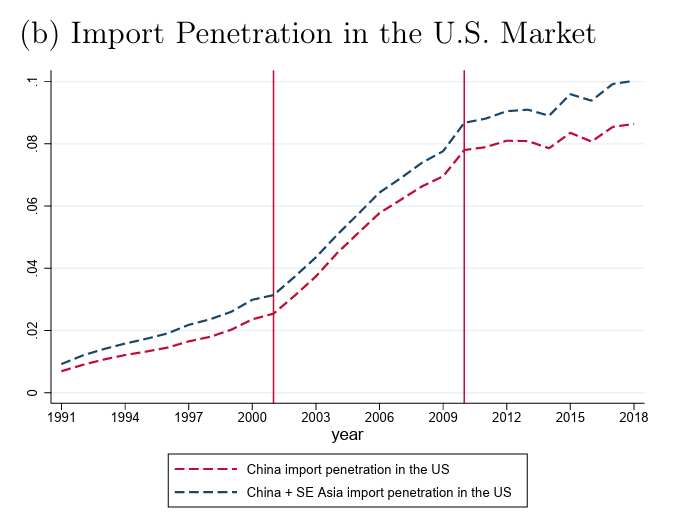
\includegraphics[width=\linewidth]{figs/china-trade-shock-penetration.png} 
        \caption{Source: \href{https://www.nber.org/system/files/working_papers/w29401/w29401.pdf}{Autor, Dorn \& Hanson (2021)}}

\end{figure}
\end{column}%
\hfill%
\begin{column}{.55\textwidth}
{\small
\begin{wideitemize}
    \item China's share in world manufacturing exports rose from 3.1\% in 1991 to 17.6\% in 2015

    \item China's share in total absorption (domestic use) in the US increased from  ~2\% to ~8\%

    \item US regions more different in terms of industrial composition

    \item China import competition was higher in manufacturing
    
    \item $\implies$ Regions with large manufacturing employment hit harder
    
\end{wideitemize}
}
\end{column}%
\end{columns}

\end{frame}

\begin{frame}{China trade shock over space}

\begin{figure}
    \centering
    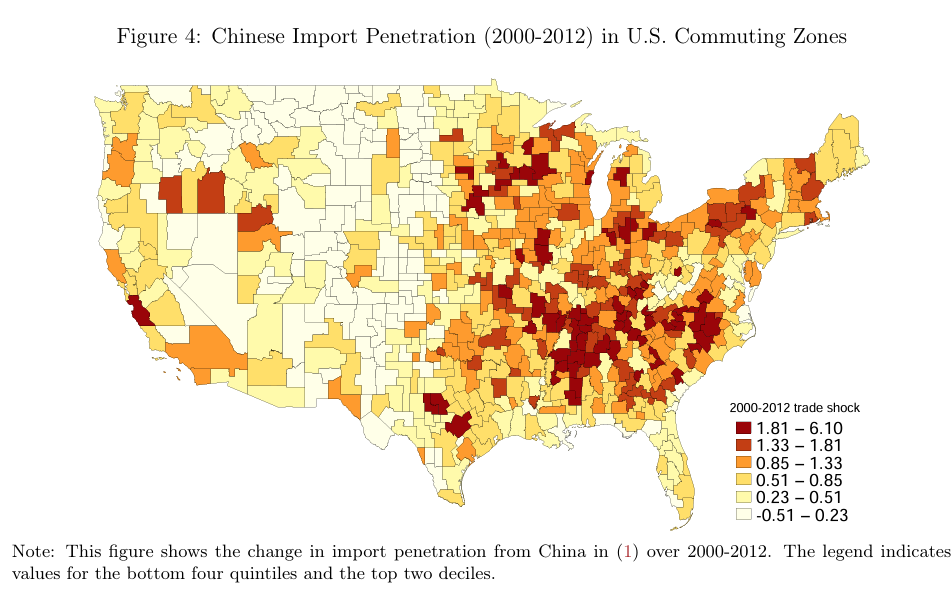
\includegraphics[width=0.75\linewidth]{figs/china-trade-shock-penetration-map.png}  
    \caption{Source: \href{https://www.nber.org/system/files/working_papers/w29401/w29401.pdf}{Autor, Dorn \& Hanson (2021)}}
\end{figure}

\end{frame}


\begin{frame}{Distributional effects of the China trade shock over labor}


\begin{columns}[T] % align columns
\begin{column}{.45\textwidth}
\centering
  \makebox[\linewidth][c]{
    \resizebox{\linewidth}{!}{
    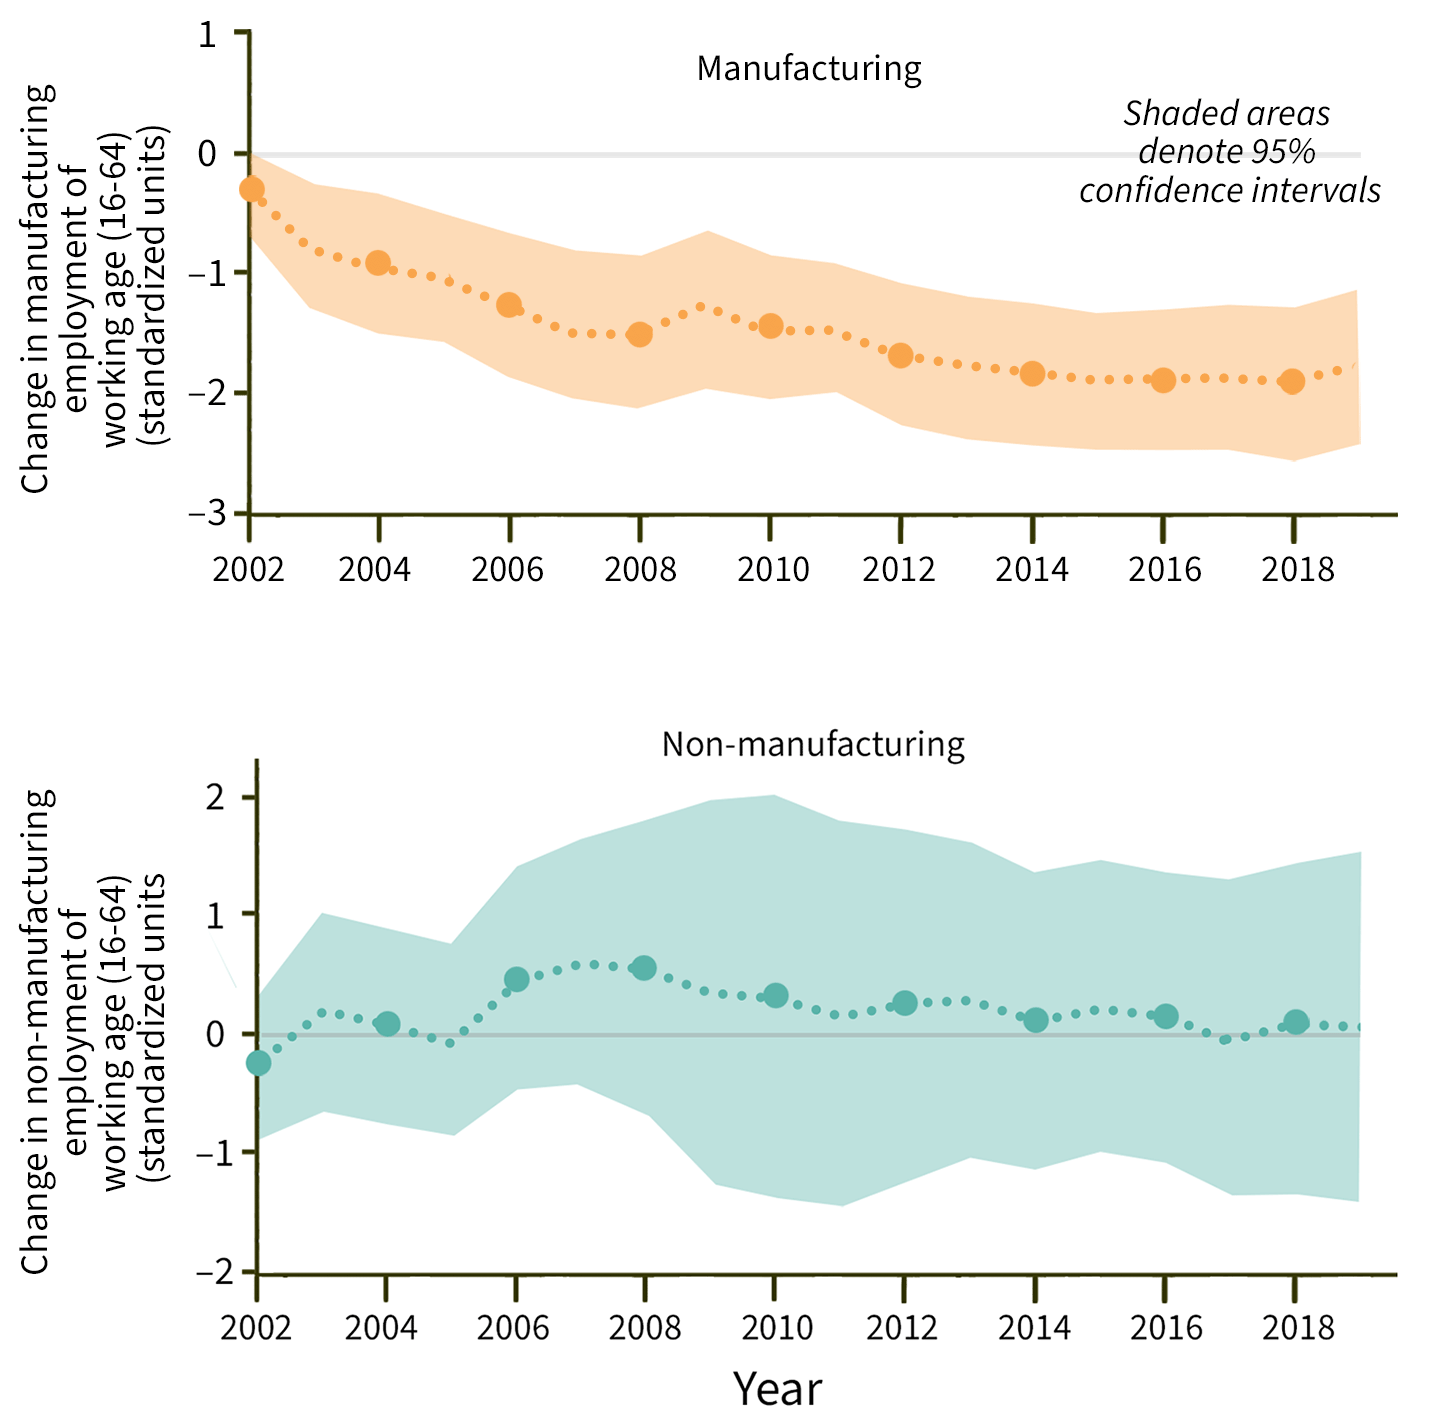
\includegraphics[width=\linewidth]{figs/shock_fig_1a-b_3.png} 
      }
    }
    \vspace{12pt}
    { \scriptsize
    Source: \href{https://www.nber.org/system/files/working_papers/w29401/w29401.pdf}{Autor, Dorn \& Hanson (2021)}
    }
\end{column}%
\hfill%
\begin{column}{.55\textwidth}
{\small
\begin{wideitemize}

    \item US regions more exposed to Chinese import competition saw (relative) losses in manufacturing employment growth

    \item Effects persist many years into the future, due to frictions for labor mobility

    \item There were winners and losers due to trade integration...

    \item Were gains larger the costs?

    
\end{wideitemize}
}
\end{column}%
\end{columns}

\end{frame}

\begin{frame}{Distributional effects of the China over income}


\begin{columns}[T] % align columns
\begin{column}{.65\textwidth}
\centering
  \makebox[\linewidth][c]{
    \resizebox{\linewidth}{!}{
    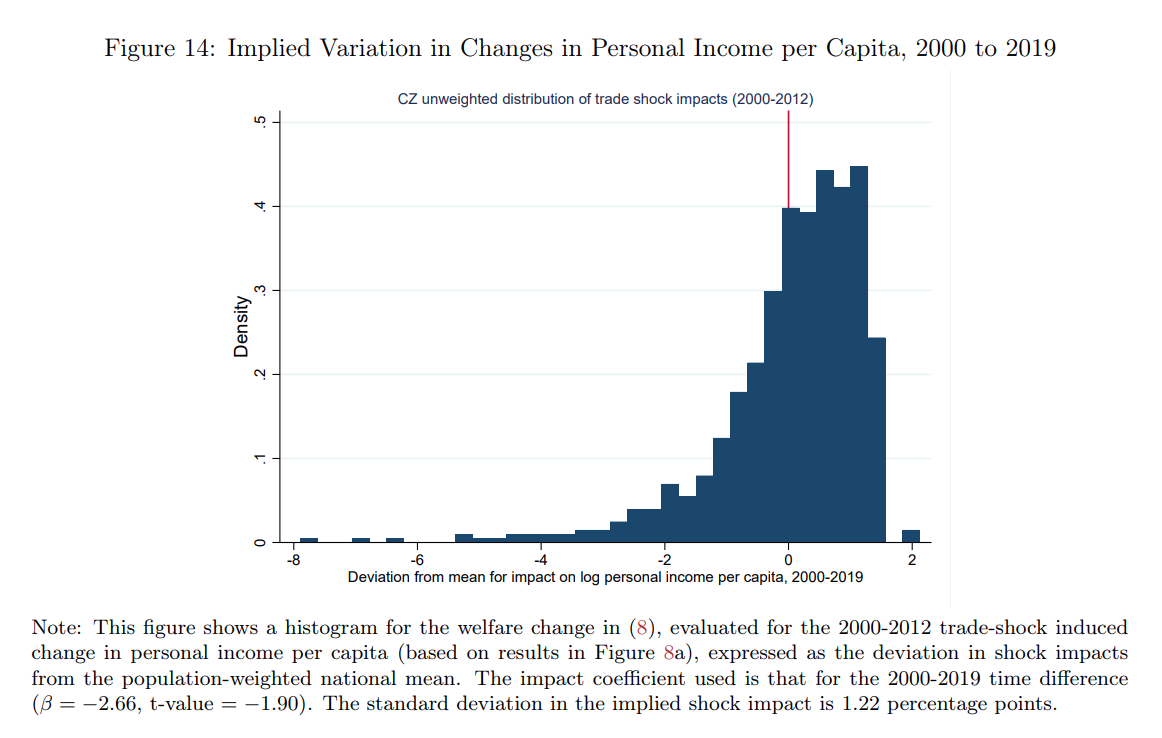
\includegraphics[width=\linewidth]{figs/china-trade-shock-prices.png} 
      }
    }
    \vspace{12pt}
    { \scriptsize
    Source: \href{https://www.nber.org/system/files/working_papers/w29401/w29401.pdf}{Autor, Dorn \& Hanson (2021)}
    }
\end{column}%
\hfill%
\begin{column}{.35\textwidth}
{\small
\begin{wideitemize}

    \item The increase in China's imports decreased prices by about  1.25\% in the US

    \item Putting the effect on income (negative) and on prices (positive), real income increased for \~94\% of Americans

    
\end{wideitemize}
}
\end{column}%
\end{columns}

\end{frame}



\begin{frame}{Distributional effects of the China over welfare}


\begin{columns}[T] % align columns
\begin{column}{.65\textwidth}
\centering
  \makebox[\linewidth][c]{
    \resizebox{\linewidth}{!}{
    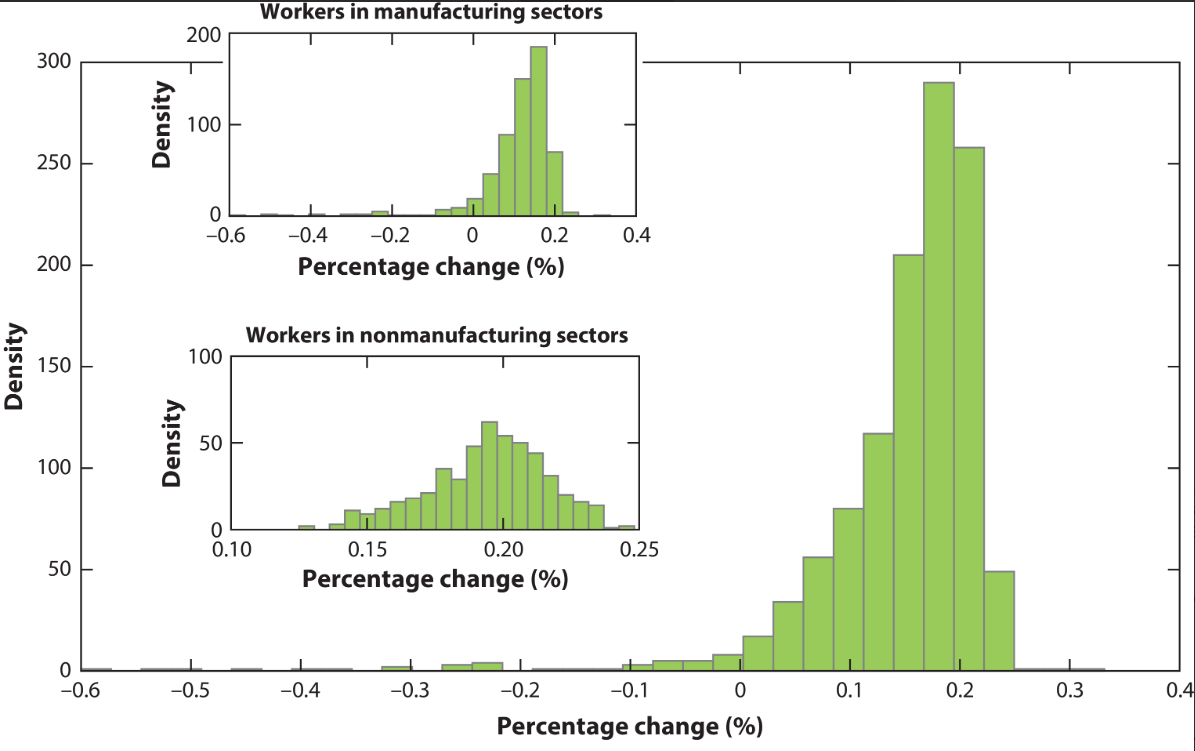
\includegraphics[width=\linewidth]{figs/china-trade-shock-welfare.png} 
      }
    }
    \vspace{12pt}
    { \scriptsize
    Source: \href{https://www.annualreviews.org/content/journals/10.1146/annurev-economics-082222-082019}{Caliendo \& Parro (2023)}
    }
\end{column}%
\hfill%
\begin{column}{.35\textwidth}
{\small
\begin{wideitemize}

    \item But this masks substantial heterogeneity across regions and sectors

    \item Gains were concentrated in the non-manufacturing sector (most of population)

    \item Manufacturing sector experienced large contractions

    \item Regions that were large manufacturing hubs (think Detroit) were affected
    
\end{wideitemize}
}
\end{column}%
\end{columns}

\end{frame}

\begin{frame}{The politics of the China trade shock}

\begin{columns}[T] % align columns
\begin{column}{.35\textwidth}
\centering
  \makebox[\linewidth][c]{
    \resizebox{\linewidth}{!}{
    
\includegraphics[width=\linewidth]{figs/death-by-china.jpg} 
      }
    }
    \vspace{12pt}
    { \scriptsize
    Source: \href{https://www.annualreviews.org/content/journals/10.1146/annurev-economics-082222-082019}{Caliendo \& Parro (2023)}
    }
\end{column}%
\hfill%
\begin{column}{.65\textwidth}
{\small
\begin{wideitemize}

    \item Peter Navarro
    \begin{itemize}
        \item Senior counselor for trade and manufacturing to President Trump
        \item Retired Econ Professor, UC Irvine
        \item Harvard PhD, 1986 (not on trade)
    \end{itemize}

    \vspace{12pt}


        \begin{quote}
        ``The defining moment in American economic history is when Bill Clinton lobbied to get China into the World Trade Organization. It was the worst political and economic mistake in American history in the last 100 years.'' -- Navarro \& Autry, Death by China 
    \end{quote}

    \vspace{12pt}

    \begin{quote}
        ``Tariffs are tax cuts. Tariffs are jobs. Tariffs are national security. Tariffs are great for America. Tariffs will make America great again.'' -- Peter Navarro on Fox News, 2025 
    \end{quote}
    
\end{wideitemize}
}
\end{column}%
\end{columns}

\end{frame}


\begin{frame}{The politics of the China trade shock}

\begin{columns}[T] % align columns
\begin{column}{.50\textwidth}
\centering
  \makebox[\linewidth][c]{
    \resizebox{\linewidth}{!}{
    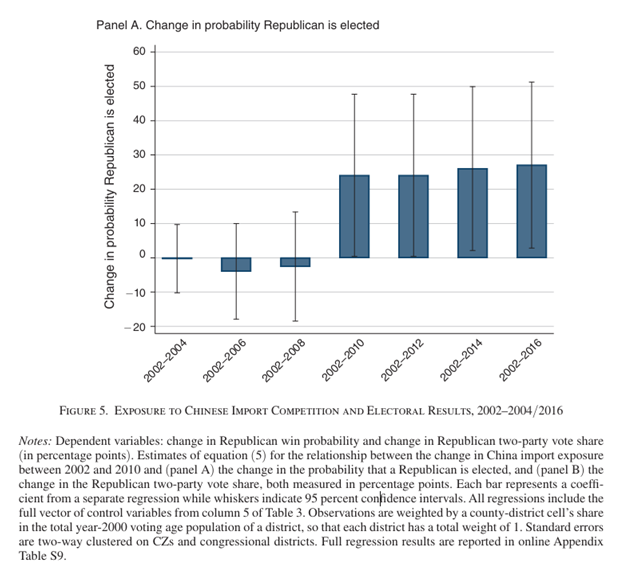
\includegraphics[width=\linewidth]{figs/electoral-outcomes-trade-shock.png} 
      }
    }
    \vspace{12pt}
    { \scriptsize
    Source: \href{https://www.aeaweb.org/articles?id=10.1257/aer.20170011}{Autor, Dorn, Hanson \& Majlesi (2020)}
    }
\end{column}%
\hfill%
\begin{column}{.50\textwidth}
{\small
\begin{wideitemize}

    \item Evidence suggests \textit{aggregate gains} but \textit{distributional consequences} of trade shock

    \item Regions more exposed to Chinese import competition were more likely to turn Republican

    \item In polarized environments, distributional impacts -- even if not large -- can have large consequences 
   
\end{wideitemize}
}
\end{column}%
\end{columns}

\end{frame}

\begin{frame}{Another example: China trade shock and Brexit}

\begin{figure}
    \centering
    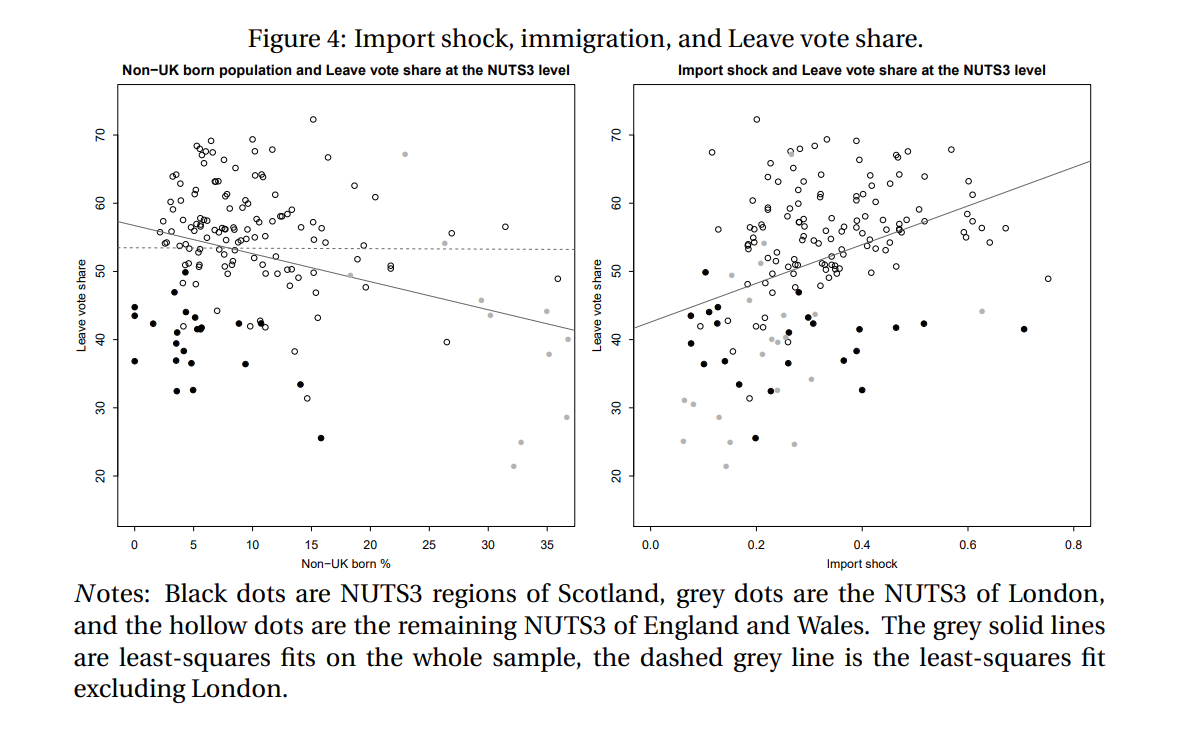
\includegraphics[width=0.75\linewidth]{figs/brexit-trade-shock.png}  
    \caption{Source: \href{https://www.cambridge.org/core/journals/american-political-science-review/article/abs/global-competition-and-brexit/C843990101DB9232B654E77130F88398}{Colantone \& Stanig (2018)}}
\end{figure}

\end{frame}

\begin{frame}{Economic consequences of Brexit}

\begin{figure}
    \centering
    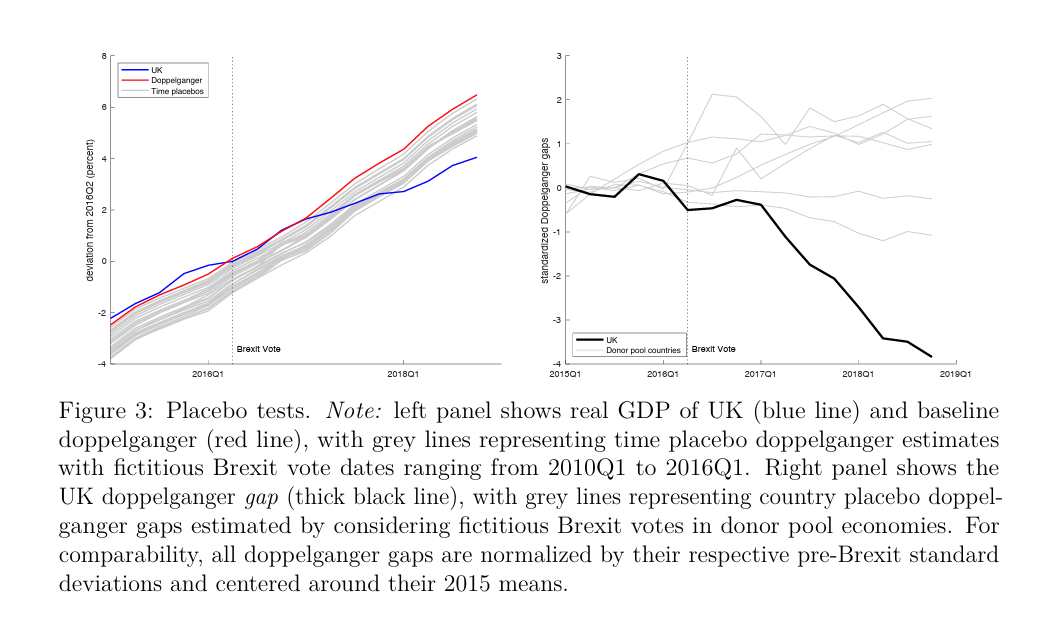
\includegraphics[width=0.75\linewidth]{figs/brexit-sc.png}  
    \caption{Source: \href{https://https://academic.oup.com/ej/article-abstract/129/623/2722/5506774}{Born, Müller, Schularick \& Sedláček (2019)}}
\end{figure}

\end{frame}

\begin{frame}{Risks of Trade Decoupling}

\begin{wideitemize}
    \item What are the risks that the world splits into a Cold War like scenario?
    \item The economic literature calls that ``trade decoupling''
    \item How bad could it be?
    \item Through the lens of the models we have seen:
    \begin{itemize}
        \item lower welfare due to more expensive prices (lower real income)
        \item distributional consequences
    \end{itemize}
    \item But also:
    \begin{itemize}
        \item lower investment
        \item less technological diffusion
        \item less innovation (market size)
        \end{itemize}
\end{wideitemize}


\end{frame}

\begin{frame}{Trade Decoupling along Political Lines?}

\begin{figure}
    \centering
    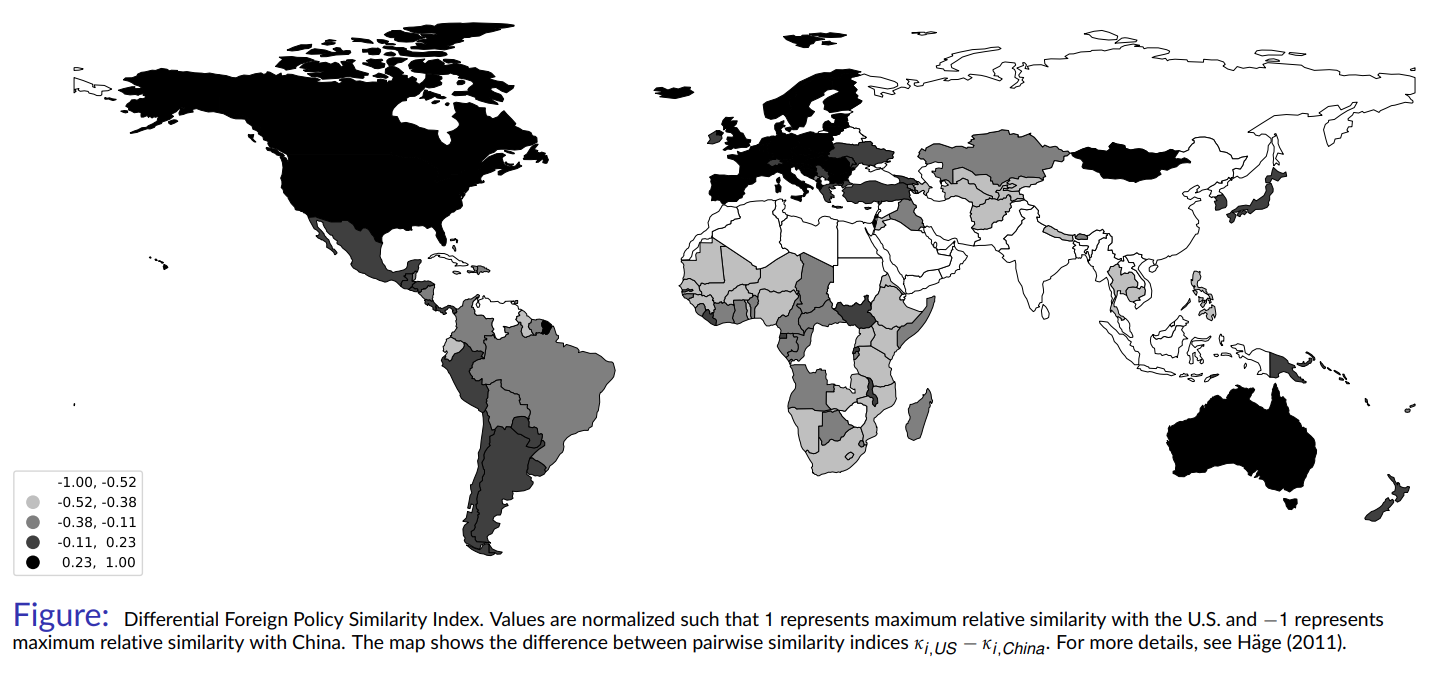
\includegraphics[width=\linewidth]{figs/decoupling-map.png} \\
    Source: \href{https://www.wto.org/english/res_e/reser_e/ersd202209_e.pdf}{Góes \& Bekkers (2022)}
\end{figure}

\end{frame}

\begin{frame}{Outcomes of Trade Decoupling}

\begin{figure}
    \centering
    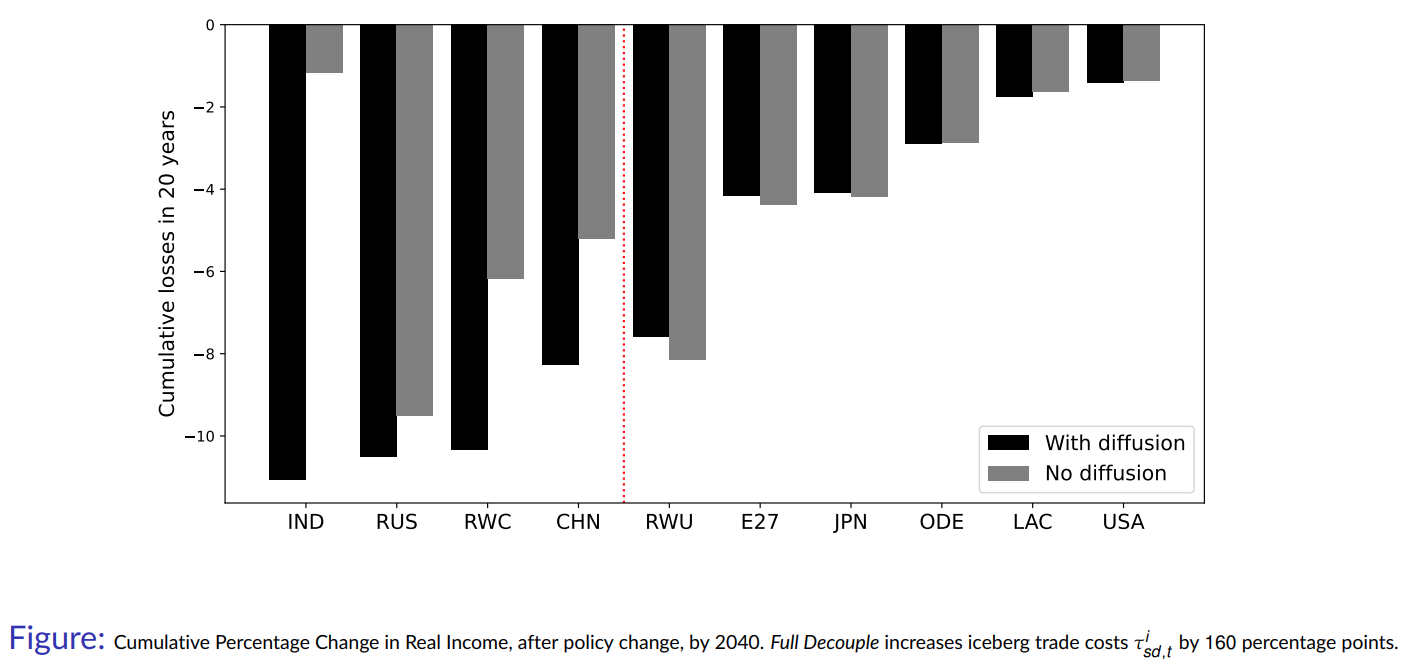
\includegraphics[width=\linewidth]{figs/decoupling-result.png} \\
    Source: \href{https://www.wto.org/english/res_e/reser_e/ersd202209_e.pdf}{Góes \& Bekkers (2022)}
\end{figure}

\end{frame}



\end{document}
